\documentclass[journal, a4paper]{IEEEtran}
\usepackage{listings}
\usepackage{fancyvrb}
\usepackage{framed}
\usepackage{float}
\usepackage{pgf}
\usepackage{tikz}
\usetikzlibrary{arrows,automata}
\usepackage{graphicx}
\usepackage{caption}
\usepackage{subcaption}
% some very useful LaTeX packages include:

\usepackage{cite}       % Written by Donald Arseneau
                        % V1.6 and later of IEEEtran pre-defines the format
                        % of the cite.sty package \cite{} output to follow
                        % that of IEEE. Loading the cite package will
                        % result in citation numbers being automatically
                        % sorted and properly "ranged". i.e.,
                        % [1], [9], [2], [7], [5], [6]
                        % (without using cite.sty)
                        % will become:
                        % [1], [2], [5]--[7], [9] (using cite.sty)
                        % cite.sty's \cite will automatically add leading
                        % space, if needed. Use cite.sty's noadjust option
                        % (cite.sty V3.8 and later) if you want to turn this
                        % off. cite.sty is already installed on most LaTeX
                        % systems. The latest version can be obtained at:
                        % http://www.ctan.org/tex-archive/macros/latex/contrib/supported/cite/

\usepackage{graphicx}   % Written by David Carlisle and Sebastian Rahtz
                        % Required if you want graphics, photos, etc.
                        % graphicx.sty is already installed on most LaTeX
                        % systems. The latest version and documentation can
                        % be obtained at:
                        % http://www.ctan.org/tex-archive/macros/latex/required/graphics/
                        % Another good source of documentation is "Using
                        % Imported Graphics in LaTeX2e" by Keith Reckdahl
                        % which can be found as esplatex.ps and epslatex.pdf
                        % at: http://www.ctan.org/tex-archive/info/

%\usepackage{psfrag}    % Written by Craig Barratt, Michael C. Grant,
                        % and David Carlisle
                        % This package allows you to substitute LaTeX
                        % commands for text in imported EPS graphic files.
                        % In this way, LaTeX symbols can be placed into
                        % graphics that have been generated by other
                        % applications. You must use latex->dvips->ps2pdf
                        % workflow (not direct pdf output from pdflatex) if
                        % you wish to use this capability because it works
                        % via some PostScript tricks. Alternatively, the
                        % graphics could be processed as separate files via
                        % psfrag and dvips, then converted to PDF for
                        % inclusion in the main file which uses pdflatex.
                        % Docs are in "The PSfrag System" by Michael C. Grant
                        % and David Carlisle. There is also some information
                        % about using psfrag in "Using Imported Graphics in
                        % LaTeX2e" by Keith Reckdahl which documents the
                        % graphicx package (see above). The psfrag package
                        % and documentation can be obtained at:
                        % http://www.ctan.org/tex-archive/macros/latex/contrib/supported/psfrag/

%\usepackage{subfigure} % Written by Steven Douglas Cochran
                        % This package makes it easy to put subfigures
                        % in your figures. i.e., "figure 1a and 1b"
                        % Docs are in "Using Imported Graphics in LaTeX2e"
                        % by Keith Reckdahl which also documents the graphicx
                        % package (see above). subfigure.sty is already
                        % installed on most LaTeX systems. The latest version
                        % and documentation can be obtained at:
                        % http://www.ctan.org/tex-archive/macros/latex/contrib/supported/subfigure/

\usepackage{url}        % Written by Donald Arseneau
                        % Provides better support for handling and breaking
                        % URLs. url.sty is already installed on most LaTeX
                        % systems. The latest version can be obtained at:
                        % http://www.ctan.org/tex-archive/macros/latex/contrib/other/misc/
                        % Read the url.sty source comments for usage information.

%\usepackage{stfloats}  % Written by Sigitas Tolusis
                        % Gives LaTeX2e the ability to do double column
                        % floats at the bottom of the page as well as the top.
                        % (e.g., "\begin{figure*}[!b]" is not normally
                        % possible in LaTeX2e). This is an invasive package
                        % which rewrites many portions of the LaTeX2e output
                        % routines. It may not work with other packages that
                        % modify the LaTeX2e output routine and/or with other
                        % versions of LaTeX. The latest version and
                        % documentation can be obtained at:
                        % http://www.ctan.org/tex-archive/macros/latex/contrib/supported/sttools/
                        % Documentation is contained in the stfloats.sty
                        % comments as well as in the presfull.pdf file.
                        % Do not use the stfloats baselinefloat ability as
                        % IEEE does not allow \baselineskip to stretch.
                        % Authors submitting work to the IEEE should note
                        % that IEEE rarely uses double column equations and
                        % that authors should try to avoid such use.
                        % Do not be tempted to use the cuted.sty or
                        % midfloat.sty package (by the same author) as IEEE
                        % does not format its papers in such ways.

\usepackage{amsmath}   % From the American Mathematical Society
                        % A popular package that provides many helpful commands
                        % for dealing with mathematics. Note that the AMSmath
                        % package sets \interdisplaylinepenalty to 10000 thus
                        % preventing page breaks from occurring within multiline
                        % equations. Use:
						%\interdisplaylinepenalty=2500
                        % after loading amsmath to restore such page breaks
                        % as IEEEtran.cls normally does. amsmath.sty is already
                        % installed on most LaTeX systems. The latest version
                        % and documentation can be obtained at:
                        % http://www.ctan.org/tex-archive/macros/latex/required/amslatex/math/



% Other popular packages for formatting tables and equations include:

%\usepackage{array}
% Frank Mittelbach's and David Carlisle's array.sty which improves the
% LaTeX2e array and tabular environments to provide better appearances and
% additional user controls. array.sty is already installed on most systems.
% The latest version and documentation can be obtained at:
% http://www.ctan.org/tex-archive/macros/latex/required/tools/

% V1.6 of IEEEtran contains the IEEEeqnarray family of commands that can
% be used to generate multiline equations as well as matrices, tables, etc.

% Also of notable interest:
% Scott Pakin's eqparbox package for creating (automatically sized) equal
% width boxes. Available:
% http://www.ctan.org/tex-archive/macros/latex/contrib/supported/eqparbox/

% *** Do not adjust lengths that control margins, column widths, etc. ***
% *** Do not use packages that alter fonts (such as pslatex).         ***
% There should be no need to do such things with IEEEtran.cls V1.6 and later.

\bibliography{reference_list}
% Your document starts here!
\begin{document}

% Define document title and author
\title{EL PROBLEMA DEL AGENTE VIAJERO CON VENTANAS DE TIEMPO}
\author{\textbf{Informe}\\
\begin{tabular}[t]{c@{\extracolsep{10em}}c}
\multicolumn{2}{c}{
Jefferson Amado Pe\~na Torres\hspace*{3em} Julieth Alegria Vaca\hspace*{3em} Cindy Valencia Tenorio
}\\
%~ \multicolumn{2}{c}{
%~ 1425590\hspace*{3em}1110009\hspace*{3em}1110400
%~ }\\
\end{tabular}\\ 
Universidad del Valle\\
Escuela de ingenieria en sistemas y computacion\\
\today \\
Cali\\
}
  
\markboth{Complejidad y Optimizacion 2014}{}
\maketitle
% The Abstract
\begin{abstract}
Este informe presenta una solucion al problema del agene viajero desde un modelo
con restricciones y programacion linea,aplicados en el curso de Complejidad y Optimizacion 2014 
y presentado a Irene Tisher y Nilso Mosso, profesores de la Escuela de ingenieria de sistemas
y computacion de la Universidad del valle
\end{abstract}
% Each section begins with a \section{title} command
\section{Descripcion del problema}
Un agente viajero tiene que visitar n sitios de venta, cada uno una sola vez. Se
conoce el tiempo de desplazamiento tdij entre cada dos sitios i y j . El agente
viajero tiene que detenerse en cada sitio para visitar a sus clientes. El tiempo
requerido en cada sitio i, denominado tiempo de servicio tsi y es conocido desde
un comienzo. Un inconveniente en la vida real es que el agente viajero no puede
visitar a sus clientes cuando más le conviene a él, sino cuando su cliente lo puede
atender. Por ello en cada sitio está denida una ventana de tiempo, [ai , bi ] donde
ai denota el momento más temprano y bi el momento más tarde en que el agente
viajero puede ser recibido por el cliente en el sitio i. El agente viajero sí puede
llegar más temprano que ai al sitio i pero tiene que asumir en este caso un
tiempo de espera (no será atendido antes de ese momento). El agente viajero
no puede llegar más tarde que bi al sitio i.
El problema del agente viajero con ventanas de tiempo consiste en planear las
visitas del agente dados los sitios y sus ventanas de tiempo, los tiempos de
desplazamiento entre sitios y el sitio de origen minimizando el tiempo total
requerido para atender a los clientes en los n sitios y regresar al sitio de origen,
respetando las ventanas de tiempo.

% Main Part
\section{Modelado del problema}

Considere un conjunto de nodos \textbf{N}= \(\left \{ 1, . . . n, \right \}\) 
que seran visitados donde el nodo origen y el nodo destino seran el mismo nodo
pues el \textit{ problema del agente viajero } \textbf{TSP} posee una estrecha relacion
con el \textit{Camino hamiltoniano} \cite{hamdef} que es definido como una sucesion de aristas 
adyacentes, que visita todos los vertices del grafo una sola vez.\\

El\textit{ problema del agente viajero con ventanas de tiempo } \textbf{TSPTW} es una variante del 
\textit{ problema del agente viajero } \textbf{TSP} que tiene asociado a cada nodo
\textit{i} \(\in\) \textbf{V}  una ventana de tiempo \( w_{i}= [a_{i},b_{i}]\), 
donde cada par de vertices estan unidos por una arista, es decir, 
contiene todas las posibles aristas \textbf{A} y cada arista tiene asociado 
un valor no-negativo que se el tiempo \(td_{i,j}\).

El \textit{ problema del agente viajero con ventanas de tiempo } es el problema de encontrar
una ruta de minimo costo visitando un conjunto de nodos solo una vez dentro de las 
ventana de tiempo descritas en cada nodo. El problema generalizado por el \textit{problema
del agente viajero} \cite{tspdef} es \textbf{NP-hard} y \textbf{Savelsbergh 1958} \cite{HOP90} 
mostro que encontrar una solucion factible del TSPTW es \textbf{NP-completo} 
%~ , se asume que este tiempo 
%~ incluye el tiempo de servicio y el tiempo en el nodo \textit{i}, es decir 
%~ \textbf{\(t_{i,j}\)}= \textbf{\(td_{i,j}\)} + \textbf{\(ts_{i}\)}, para todos los 
%~ \textit{i} \(\in\) \( N\cup \left \{ o\right \}\). 
%~ Un arco (i,j) es definido en el conjunto
%~ de los A si mantien la siguiente condicion:
%~ \[
	%~ a_{i}+t_{i,j}\leq b_{j}; \> 
	%~ \textit{i}  \in  N\cup \left \{ o\right \}; \>
	%~ \textit{j} \in N\cup \left \{ d\right \} ; \>
	%~ i\neq j
%~ \]

\section{Formulacion matematica}

En el modelo utiliza variables como: \(X_{i,j},  (i,j) \in A \)  que es una variable binaria 
y que indica indica el flujo entre los nodos \(\textit{i} \to \textit{j}\) y \(s_{i}\)
que es una variables de tiempo tal que \(s_{i} \geq a_{i} \wedge  s_{i} \leq b_{i} \). y
la variable espera \(\varepsilon \) que adquiere valor cuando se llega a un nodo antes de que la 
ventana de tiempo [\(a_{i}\)]  sea abierta .\\ \\
Para la formulacion del problema se requirio de dos nodos especiales o virtuales 
denominados "origen" \textbf{o} y "destino"  \textbf{d}, sea \textbf{V}=\( N\cup \left \{ o,d \right \}\). 
Una permutacion permitida de nodos que se cumple todas las restricciones de las ventanas de tiempos,
puede estar representada teniendo en cuenta los nodos artificiales \textbf{o} y \textbf{d}, 
que tienen tiempos de servicio \(ts_{o} =0\) y \(ts_{d}=0\)  y tiempos de desplazamiento 
\(td_{o,j} =1\) y \(td_{i,d}=1\), donde el \textbf{o} 
posee aristas desde el hacia todos los nodos y todos lo nodos a \textbf{d},
estos nodos poseen ventanas de tiempo \( W_{o}= [a_{o},a_{o}]\) y \( W_{d}= [a_{d},a_{d}]\) 
donde \(a_{o} = 0 \)  un valor menor que todos los \(a_{i}\) los otros nodos y 
\(a_{d} = M\) un valor mayor que todos los \(b_{j}\) de los otros nodos.
El objetivo a resolver es minimizar el tiempo de recorrido teninedo en cuenta el tiempo de servicio y
el tiempo de desplazamiento denomindado como \(  Q_{i,j} = ts_{i}+ td_{i,j} \). \\\\
La ruta de costo minimo  inicia en el intervalo de tiempo que inicia en la ventana
\(\left[ a_{0}, b_{0} \right]\) que tiene valores desde el archivo (0,0)
como nodo origen, visitando exactamente una vez todos los nodos \cite{tspdef} 
que estan en \textbf{N} teniendo en cuenta las restriciones de las ventanas 
de tiempo en cada nodo se formula como:
%~ \\\\ \\
\[ X_{i,j} = \left\{ \begin{array}{ll}
         1 & \mbox{Si el el nodo j es visitado despues de visitar i};\\
         0 & \mbox{en otro caso}.\end{array} \right. \] 
%~ \\
%~ \begin{lstlisting}[frame=single]
\begin{equation} 
 minimizar \> Z= \sum_{\substack{(i,j)\in A}} Q_{i,j} X_{i,j} + \sum_{\substack{(i,j)\in A}} \varepsilon _{i,j}
\end{equation}
sujeto a:
%~ http://opti-lineal.blogspot.com/2013/04/agente-viajero-simple-y-multiple-grupo-5.html
%~ Para garantizar que se sale de cada ciudad exactamente una vez
\begin{equation} 
\sum_{\substack{j=0,i\neq j}} X_{i,j} = 1 \> \> \> 
\forall i \> \in \textbf{V} - \left \{ q \right \},
%~ \forall i \> \in \left \{ 1,...,n\right \}
\end{equation}
%~ Para garantizar que se llega a cada ciudad exactamente una vez
\begin{equation} 
\sum_{\substack{i=0,i\neq j}} X_{i,j} = 1 \> \> \>
\forall j \> \in \textbf{V} - \left \{ p \right \},
%~ \forall j \> \in \left \{ 1,...,n+1\right \}
\end{equation}
%~  no ciclos
\begin{equation} 
u_{i}-u_{j}+NX_{i,j} \leq N-1
\end{equation}
%~  inecuaciones
\begin{equation} 
%~ s_{i} + \left (td_{i,j} + ts_{i} \right) -e_{i} - s_{j} \leq \left ( 1 - X_{i,j} \right ) M_{i,j},
s_{i} + Q_{i,j} -e_{i} - s_{j} \leq \left ( 1 - X_{i,j} \right ) M_{i,j},
\end{equation}
%~  Ventanas de tiempo
\begin{equation} 
a_{i}\leq s_{i} \leq b_{i} \> \forall i \> \in \> V,
\end{equation}
%~ esperas s2 - 6 - s1 + e1 + 100 x12 - 100 <= e12;
\begin{equation} 
%~ s_{j} - \left (td_{i,j} + ts_{i} \right) + e_{i} - s_{i} + M X_{i,j} - M \leq \varepsilon _{i,j},
s_{j} - Q_{i,j} + e_{i} - s_{i}  \leq \varepsilon _{i,j} - M (X_{i,j} - 1),
\end{equation}
%~  Variables
\begin{equation} 
X_{i,j} \in \left \{ 0,1 \right \} \> \forall (i,j) \> \in \> A,
\end{equation}
%~ \end{lstlisting}
En  (1) la variable \(X_{i,j}\)  es \textbf{1} si el arco (i,j) es usado en la ruta optima  
es \textbf{0} en otro caso, el valor \(  Q_{i,j} = ts_{i}+ td_{i,j} \)  es un numero 
que indica el valor entre (i,j) y \( \varepsilon _{i,j} \)es la espera generada en la arista (i,j).\\
Las restriccion (2) obliga a que desde un nodo solo se tome una arista hacia otro nodo,
la (3) obliga a que desde otro nodo solo se tome una arista a este nodo,
ambas aseguran que una ruta desde \textbf{o} hasta \textbf{d} sea un ciclo dirigido que 
pasa por todos lo nodos de \textbf{N} y que la variable \(X_{i,j}\)
con valor en 1 indique las transiciones  \(\textit{i} \to \textit{j}\) entre los nodos. 
La restriccion (4) impide que se generen ciclos, esta plantea un conjunto de ecuaciones donde cada valor
\( u_{i} \) obliga a que se cubra todas las ciudades y no dos o más caminos disjuntos.

la restriccion(5) aseguran que una solucion respete las ventanas de tiempo en cada nodo y que
se asegure la factibilidad del tiempo planeado,cuando \( b_{i,j} + Q_{i,j} \leq a_{i,j} \), es decir,
el mejor de los caso las restricciones siempre seran satisfechas para cualquier 
valor de \( s_{i}\)  y de \(s_{j}\), para el otro caso puede que no halla solucion,la restriccion (6) asegura que 
el momento de inicial es servicio en el nodo i este dentro del marco de la ventana de cada nodo \textbf{N} haciendo que sea 
factible o no la solucion,la restricion (7) modela la espera, si se llega a un nodo \textit{i} antes de la apertura de la
ventana se debe esperar y el tiempo gastado en ese nodo sera la suma 

la restriccion (8) indica que la variable \(X_{i,j}\) solo puede tomar valores 0 y 1 (\textbf{binaria})

%~ \subsection{Estrategia para evitar ciclos}
%~ Los ciclos se prohibieron con las restricciones de la forma (\(X_{1,2}+ X_{2,1}\leq 1\))
%~ que impide la ruta mostrada en la figura (b), (\(X_{1,2}+ X_{2,3}+ X_{3,1}\leq 2\))
%~ que impide la ruta mostrada en la figura (c), (\(X_{1,2}+ X_{2,3}+ X_{3,4} +X_{4,1} = 4\))
%~ que asegura que el unico ciclo sea igual a \textbf{N} en caso del ejemplo sea 4.
%~ La parte derecha de estas restricciones son todas las combinaciones desde un nodo a otro que pueden dejar nodos  por fuera de la solucion ej.para una 
%~ instancia de 4 nodos una solucion no podra ser \( 1 \to 2\to 3\to 1 \) 
%~ pues quedaria sin visitar el nodo 4 pero la restriccion (\(X_{1,2}+ X_{2,3}+ X_{3,1}\leq 2\)) impedira que 
%~ este ciclo haga parte de la solucion obligando a que \( 1 \to 2\to 3 \) pero no tomar la ruta a 1
%~ \begin{figure}[H]
%%~ \centering
%~ \subfloat[]{
%~ \begin{tikzpicture}[->,>=stealth',shorten >=1pt,auto,node distance=3cm,thick,main node/.style={circle,fill=blue!20,draw,font=\sffamily\Large\bfseries},scale=0.75]
  %~ \tikzset{LabelStyle/.style = {fill=white,sloped}}
  %~ 
  %~ \node[main node] (1) {1};
  %~ \node[main node] (2) [below left of=1] {2};
  %~ \node[main node] (3) [below right of=2] {3};
  %~ \node[main node] (4) [below right of=1] {4};
%~ 
  %~ \path[every node/.style={font=\sffamily\small}]
    %~ (1) edge node [left ] 			 [LabelStyle]{x14} (4)
        %~ edge [bend right] node[left] [LabelStyle]{x12} (2)
        %~ edge [bend left ] node[left] [LabelStyle]{x13} (3)
    %~ (2) edge node [right] 			 [LabelStyle]{x21} (1)
        %~ edge [bend right] node[right] [LabelStyle]{x24} (4)
        %~ edge [bend right] node[left] [LabelStyle]{x23} (3)
    %~ (3) edge node [right] 			 [LabelStyle]{x32} (2)
        %~ edge [bend right] node[right][LabelStyle]{x34} (4)
        %~ edge [bend left ] node[left] [LabelStyle]{x31} (1)
    %~ (4) edge [bend right] node[left] [LabelStyle]{x42} (2)
        %~ edge node [left ] 			 [LabelStyle]{x43} (3)
        %~ edge [bend right] node[right][LabelStyle]{x41} (1);
%~ \end{tikzpicture}        
%~ }
%~ \subfloat[]{
%~ \begin{tikzpicture}[->,>=stealth',shorten >=1pt,auto,node distance=3cm,thick,main node/.style={circle,fill=blue!20,draw,font=\sffamily\Large\bfseries},scale=0.75]
  %~ \tikzset{LabelStyle/.style = {fill=white,sloped,text=red}}
  %~ \node[main node] (1) {1};
  %~ \node[main node] (2) [below left of=1] {2};
  %%~ \node[main node] (3) [below right of=2] {3};
  %%~ \node[main node] (4) [below right of=1] {4};
  %~ 
  %~ \path[every node/.style={font=\sffamily\small}]
    %~ (1) edge [bend right] node[left] [LabelStyle]{x12} (2)  
    %~ (2) edge [bend right] node[right][LabelStyle]{x21} (1);
  %~ 
%~ \end{tikzpicture}
%~ }
%~ \subfloat[]{
%~ \begin{tikzpicture}[->,>=stealth',shorten >=1pt,auto,node distance=3cm,thick,main node/.style={circle,fill=blue!20,draw,font=\sffamily\Large\bfseries},scale=0.75]
  %~ \tikzset{LabelStyle/.style = {fill=white,sloped,text=red}}
  %~ \node[main node] (1) {1};
  %~ \node[main node] (2) [below left of=1] {2};
  %~ \node[main node] (3) [below right of=2] {3};
  %%\node[main node] (4) [below right of=1] {4};
  %~ \path[every node/.style={font=\sffamily\small}]
    %~ (1) edge [bend right] node[left] [LabelStyle]{x12} (2)
    %~ (2) edge [bend right] node[left] [LabelStyle]{x23} (3)
    %~ (3) edge [bend left ] node[left] [LabelStyle]{x31} (1);
  %~ 
%~ \end{tikzpicture}
%~ }
%~ \subfloat[]{
%~ \begin{tikzpicture}[->,>=stealth',shorten >=1pt,auto,node distance=3cm,thick,main node/.style={circle,fill=blue!20,draw,font=\sffamily\Large\bfseries},scale=0.75]
  %~ \tikzset{LabelStyle/.style = {fill=white,sloped,text=red}}
  %~ \node[main node] (1) {1};
  %~ \node[main node] (2) [below left of=1] {2};
  %~ \node[main node] (3) [below right of=2] {3};
  %~ \node[main node] (4) [below right of=1] {4};
    %~ \path[every node/.style={font=\sffamily\small}]
    %~ (1) edge [bend right] node[left] [LabelStyle]{x12} (2)
    %~ (2) edge [bend right] node[left] [LabelStyle]{x23} (3)
    %~ (3) edge [bend right] node[left] [LabelStyle]{x34} (4)
    %~ (4) edge [bend right] node[left] [LabelStyle]{x41} (1);
  %~ 
%~ \end{tikzpicture}
%~ }
%~ \end{figure}
\subsection{Estrategia de los nodos artificiales}
Los nodos artificiales permiten una solucion factible desde un nodo \textbf{i} a el mismo \textbf{i},
pues es el unico ciclo permitido (\textit{Hamilton path} \cite{hamdef}) las variables \(X_{o,j}\) y \(X_{i,d}\) estaran en 
la solucion permitiendo que desde el nodo origen se pueda ir a cualquier otro nodo, pero el no es alcanzable para 
ninguno, y el destino alcanzable para todos pero que de el no se puede continuar con la ruta pues es el destino\\
\\
La importancia de estos nodos es que cualquier nodo puede tener como ventana de tiempo 
\( W_{i}= [0,0] \> \forall i \in N\) el
modelo podra indicar que la ruta debe iniciar por este nodo i y debe terminar en el mismo.\\

Si la ruta optima inicia por el nodo con id 1, dado que la ventana en este punto sea \( W_{1}= [0,0]\) y supuniendo la ruta que se
describe en el grafico la ruta para el lpsolve sera \textbf{\(P \to 1\to 2\to 3\to 4\to Q\)}, 
donde xP1 y x4Q tiene valor 1 y son asu vez el nodo por donde se inicio y donde se termino la ruta es decir 1 \\
\begin{figure}[H]
\centering
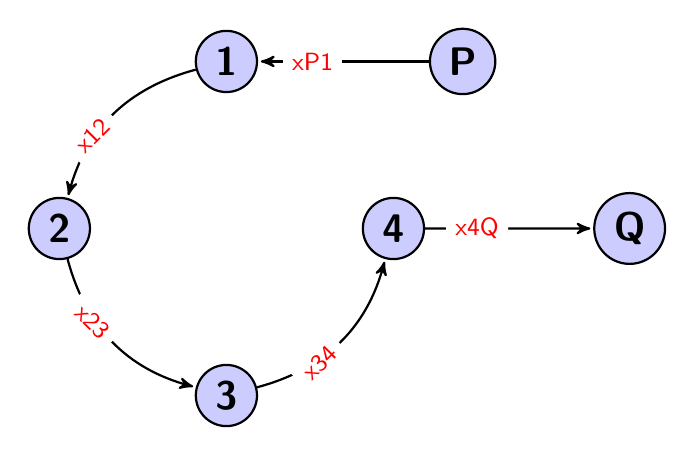
\begin{tikzpicture}[->,>=stealth',shorten >=1pt,auto,node distance=3cm,thick,
  main node/.style={circle,fill=blue!20,draw,font=\sffamily\Large\bfseries},scale=0.15]
  \tikzset{LabelStyle/.style = {fill=white,sloped,text=red}}
  \node[main node] (1) {1};
  \node[main node] (2) [below left of=1] {2};
  \node[main node] (3) [below right of=2] {3};
  \node[main node] (4) [below right of=1] {4};
  \node[main node] (5) [right of=1]{P};  
  \node[main node] (6) [right of=4]{Q}; 
     
    \path[every node/.style={font=\sffamily\small}]
    (5) edge node[left] [LabelStyle]{xP1} (1)
    (4) edge node[left] [LabelStyle]{x4Q} (6)
    (1) edge [bend right] node[left] [LabelStyle]{x12} (2)
    (2) edge [bend right] node[left] [LabelStyle]{x23} (3)
    (3) edge [bend right] node[left] [LabelStyle]{x34} (4);
    %~ %%~ (4) edge [bend right] node[left] [LabelStyle]{x41} (1);
\end{tikzpicture}
\end{figure}
El haber agregado estos nodos acarreo con algunas sumas en el valor objetivo, pues como la ruta verdaderamente 
no va al nodo de origen, las aristas \textbf{xP*} y \textbf{x*Q} tiene un \( Q_{i,j}=1 \), es decir se suma un
al valor objetivo y no el valor real de la arista.

\section{implementacion}
El \textbf{Univalle TSPTW Solver} es un aplicativo que implementa el modelo
propuesto en este informe, creando de manera dimanica las restricciones segun
la instancia de entrada y utilizando las librerias de \textbf{lpsolve} \cite{lpdef} 
con las que genera una solucion al problema TSPTW.\\
El codigo fuente esta escrito en Java (lenguaje de programacion)\cite{javadef} y se encuentra
adjunto a este informe,\textbf{Univalle TSPTW Solver} es imlementado para
\textbf{linux} y usa \textbf{Make} para la gestion de dependencias.

\textbf{Univalle TSPTW Solver} se ha probado y comparado con las instancias de 
Dumas Benchmarks \cite{HOP93} y Silva-Urrutia Benchmarks\cite{HOP91} creando una 
lectura y transformacion de instancias a las propuestas en el proyecto, obteniendo
una solucion optima para 15 nodos 
La carpeta principal de \textbf{Univalle TSPTW Solver} tiene las subcarpetas:
\textbf{entrada:} Aqui reside algunos archivos de entrada para el aplicativo
\textbf{informe:} Aqui reside el informe y las graficas obtenidas de las implementacion
\textbf{src:} Aqui reside el codigo fuente en tres subcarpetas, algorithms que contiene los
algortimos que generan las restricciones y el uso del API de lpsolve, data que contiene
la lectura del archivo y el acceso a los datos y view que contiene la interfaz grafica de usuario(GUI).
\textbf{salidas:} Aqui reside la soluciones a las instancias en formato de texto plano
\textbf{lib:} Aqui reside las librerias de lpsolve para arquitecturas de 32-bits y 64-bits y el (.jar) que 
contiene el API de lpsolve
\textbf{xlpsolve:} algunos archivos en formato (.lp) que sirven para ver el modelo en ejecucion 
\textbf{doc(opcional):} Aqui reside si se genero documentacion el API de \textbf{Univalle TSPTW Solver}
\textbf{class(opcional):} Aqui reside si se compilo los (.class) o bycode generado por java
\textbf{bin(opcional):} Aqui reside si se genero un (.jar) con el ejecutable de \textbf{Univalle TSPTW Solver}
\subsubsection{compilacion}
\textbf{Univalle TSPTW Solver} utiliza \textbf{Make} en una emulador de terminal
ubicandose en la carpeta del proyecto se teclea \textbf{make} y este comando generara
lo necesario para su ejecucion
\begin{figure}[H]
\centering
  \includegraphics[width=70mm]{emulador.png}
  \caption{compilacion en xterm usando el comando make}
  \label{usando el comando make}
\end{figure}
\subsubsection{ejecutar Univalle TSPTW Solver}
\textbf{Univalle TSPTW Solver} utiliza \textbf{Make} en una emulador de terminal
ubicado en la carpeta del proyecto se teclea \textbf{make run} o \textbf{make debug}
ejecutara el aplicativo en modo simple en el que solo entrega resultados
o en modo depuracion que muestre en el emulador de terminal
las interaciones que va haciendo paso a paso
\begin{figure}[H]
\centering
\includegraphics[width=70mm]{debug.png}
  \caption{modo depuracion}
  \label{usando el comando make debug}
\end{figure}
\subsubsection{interfaz grafica de usuario GUI}
Para cargar una nueva instancia se debe pulsar el boton de abrir (open)
y se mostrara un grafo totalmente conectado,es decir de un nodo a todos,
cada nodo presentara un color azul y con un texto \textbf{ c:ID time-service \([a_{i},b_{i}]\) }
este se podra mover con el raton y su ubicaion es aleatoria,
las aristas entre los nodos puede ser de varios colores y encima de estas aparece el tiempo de viaje 
entre un par de nodos \(td_{i,j} \), el numero de nodos y arista en el archivo se puede ver
en la parte inferior derecha en espacio log.
\begin{figure}[H]
\centering
\includegraphics[width=70mm]{front.png}
  \caption{interfaz grafica de usuario GUI}
  \label{usando el comando make run}
\end{figure}
\subsubsection{Puesta en marcha}
\textbf{Univalle TSPTW Solver} despues de cargar una instancia desde un archivo
se puede ejecutar el algortimo desde el boton run y este generar en log los nodos 
que hacen parte de la solucion y el valor minimo obtenido en rojo, ademas mostrara 
en la parte superior derecha el grafico solucion
\begin{figure}[H]
\centering
\includegraphics[width=70mm]{run.png}
  \caption{modo depuracion}
  \label{}
\end{figure}
\subsubsection{documentacion}
\textbf{Univalle TSPTW Solver} esta escrito en \textbf{Java} y utiliza \textbf{Make} en una emulador de terminal
ubicado en la carpeta del proyecto se teclea \textbf{make doc} que genera la documentacion API
por medio del javadoc y este queda en la subcarpeta "doc".
\begin{figure}[H]
\centering
  \includegraphics[width=70mm]{doc.png}
  \caption{Documentacion (API) de Univalle TSPTW Solver }
  \label{usando el comando make doc}
\end{figure}
\section{Experimentos y pruebas}
\subsection{Solucion}
La respuesta a una entrada es mostrada por \textbf{Univalle TSPTW Solver} en la parte inferior derecha,
para una instancia primero el nombre del archivo de entrada,caracteristicas del archivo, 
como el numero de nodos y aristas, luego los IDs de los nodos con las rutas entre los nodos 
que hacen minima la solucion.\\
para una instancia cualquiera la forma de la solucion sera:
\begin{lstlisting}[frame=single]
(n20wX.001.txt)(162.12) 
1 -> 2, 3->6, 2->4,6-> 10,10->9,8->7,
P->2, 5->Q
\end{lstlisting}
y que podra ser guardada como un archivo de texto plano, se incluye los nodo artificial
que indica por donde inicio la ruta,\textbf{\(P\to2\)} inicio por el nodo 2 , y el nodo artificial
que inidica cual es el nodo antecesor al nodo destino, \textbf{\(5\to Q\)} antes de ir a dos pasa por 5\\
\subsubsection{Algunas instancias}
Para pruebas utilizamos algunas entradas de 4,5,6,7,8,9 nodos con ventanas factibles 
y de multiples tama\~os, ademas se probo con los archivos entregados por la profesora mencionados en la
tabla como tsptw1.txt y tsptw2.txt. Para el c\'alculo de los tiempos.\\ 
La siguiente tabla muestra los tiempos que se tarda en generar las restricciones 
\textbf{Univalle TSPTW Solver} y el tiempo que tarda el \textbf{LpSolver} en resolver la matriz
y obtener el valor objetivo, todos estos archivos se encuentran en la carpeta entrada.
\begin{figure}[H]
\centering
  \includegraphics[width=90mm]{img.png}
  \caption{Gr\'afico de los datos}
\end{figure}

\begin{center}
  \begin{tabular}{ || l | c | r ||}
    \hline
    & tiempo & tiempo \\ 
    Archivo & Restricciones & solver \\ \hline
    tsptw1.txt & 0.173ms & 0.035ms \\ \hline
    tsptw2.txt & 0.149ms & 0.115ms \\ \hline
    n4t4wX.txt & 0.040ms & 0.005ms \\ \hline
    n5t5wX.txt & 0.063ms & 0.026ms\\ \hline
    n05w05.005.txt & 0.075ms & 0.023ms\\ \hline
    n07w07.002.txt & 0.153ms & 0.162ms\\ \hline
    n08w08.003.txt & 0.129ms & 0.385ms \\ \hline
    n09w09.003.txt & 0.189ms & 1.964ms \\ \hline
    n09w09.004.txt & 0.187ms & 0.911ms \\ \hline
    n10w10.001.txt & 0.195ms & 9.747ms \\
    \hline
  \end{tabular}
\end{center}
Como puntos de referencia, se utilizaron dos formatos que en la 
mayoria de lecturas realizadas se toman como referente, \textbf{Univalle TSPTW Solver}
posee un convertidor desde estos formatos con el fin de utilizarlos como pruebas para el modelo,
dando credito a sus respectivos autores, que toman gran cuidado en mantener un formato
para las instancias de manera uniforme, esto autores y sus formatos son:\\
\subsubsection{Dumas Benchmarks \cite{HOP93}}
Un archivo o instancia presentada en el formato Dumas Benchmarks \cite{HOP93}
contiene, primero un numero que indica el numero de nodos (n) incluido en nodo destino,
luego posee posee una matrix de adyacencia 
(normalmente son los tiempos de viaje \( td_{i,j}\) entre los nodos \( i \neq j\)),
finalmente se encuentran las ventanas de tiempo para cada nodo estos fieron tomados
de la pagina de sus Benchmarks \cite{DUMASBENCH}
\subsubsection{Silva-Urrutia Benchmarks\cite{HOP91}}  
Un archivo o instancia presentada en el formato Silva-Urrutia Benchmarks\cite{HOP91}
contine,una linea comentada con el nombre del archivo, luego unas etiquetas 
CUST NO., XCOORD, YCOORD,DEMAND,[READY TIME],[DUE TIME] y [SERVICE TIME]
que acertadamente concuerdan con las necesidades del TSPTW,aunque el autor no usa
la columna DEMAND y en sus archivos no piensa tener mas de 999 nodos pues este numero
define el limite de los nodos estos fieron tomados de la pagina de sus Benchmarks \cite{SILVABENCH}

\section{Resultados computacionales}  
El modelo descrito codificado en java se ejecuto en un Intel Pentium Dual-Core Mobile T4200 a 2,0 GHz
de arquitectura de 32-bits y con la versi\'on 7 de java, En la practica el problema de agente viajero 
con ventanas de tiempo es dificil, es decir puede verificarse en tiempo polinomial 
pero no exite un algoritmo que halle una soluci\'on poco tiempo dependiedo de la instancia.
\subsection{Complejidad computacional}

\begin{center}
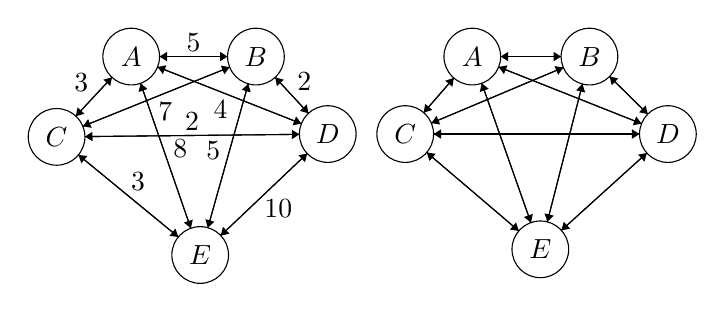
\begin{tikzpicture}[scale=0.12]
\tikzstyle{every node}+=[inner sep=0pt]
\draw [black] (17,-12.1) circle (3);
\draw (17,-12.1) node {$A$};
\draw [black] (30.2,-12.1) circle (3);
\draw (30.2,-12.1) node {$B$};
\draw [black] (9.1,-20.6) circle (3);
\draw (9.1,-20.6) node {$C$};
\draw [black] (37.8,-20.3) circle (3);
\draw (37.8,-20.3) node {$D$};
\draw [black] (24.3,-33.1) circle (3);
\draw (24.3,-33.1) node {$E$};
\draw [black] (53.1,-12.1) circle (3);
\draw (53.1,-12.1) node {$A$};
\draw [black] (65.5,-12.1) circle (3);
\draw (65.5,-12.1) node {$B$};
\draw [black] (46,-20.3) circle (3);
\draw (46,-20.3) node {$C$};
\draw [black] (73.8,-20.3) circle (3);
\draw (73.8,-20.3) node {$D$};
\draw [black] (60.3,-32.5) circle (3);
\draw (60.3,-32.5) node {$E$};
\draw [black] (20,-12.1) -- (27.2,-12.1);
\fill [black] (27.2,-12.1) -- (26.4,-11.6) -- (26.4,-12.6);
\draw (23.6,-11.6) node [above] {$5$};
\draw [black] (27.2,-12.1) -- (20,-12.1);
\fill [black] (20,-12.1) -- (20.8,-12.6) -- (20.8,-11.6);
\draw [black] (26.48,-31.04) -- (35.62,-22.36);
\fill [black] (35.62,-22.36) -- (34.7,-22.55) -- (35.39,-23.28);
\draw (32.57,-27.18) node [below] {$10$};
\draw [black] (21.98,-31.19) -- (11.42,-22.51);
\fill [black] (11.42,-22.51) -- (11.72,-23.4) -- (12.35,-22.63);
\draw (17.71,-26.36) node [above] {$3$};
\draw [black] (23.31,-30.27) -- (17.99,-14.93);
\fill [black] (17.99,-14.93) -- (17.78,-15.85) -- (18.72,-15.53);
\draw (21.41,-21.86) node [right] {$8$};
\draw [black] (25.11,-30.21) -- (29.39,-14.99);
\fill [black] (29.39,-14.99) -- (28.69,-15.62) -- (29.65,-15.89);
\draw (26.48,-22.05) node [left] {$5$};
\draw [black] (17.99,-14.93) -- (23.31,-30.27);
\fill [black] (23.31,-30.27) -- (23.52,-29.35) -- (22.58,-29.67);
\draw [black] (29.39,-14.99) -- (25.11,-30.21);
\fill [black] (25.11,-30.21) -- (25.81,-29.58) -- (24.85,-29.31);
\draw [black] (35.62,-22.36) -- (26.48,-31.04);
\fill [black] (26.48,-31.04) -- (27.4,-30.85) -- (26.71,-30.12);
\draw [black] (11.42,-22.51) -- (21.98,-31.19);
\fill [black] (21.98,-31.19) -- (21.68,-30.3) -- (21.05,-31.07);
\draw [black] (14.96,-14.3) -- (11.14,-18.4);
\fill [black] (11.14,-18.4) -- (12.05,-18.16) -- (11.32,-17.48);
\draw (12.52,-14.89) node [left] {$3$};
\draw [black] (32.24,-14.3) -- (35.76,-18.1);
\fill [black] (35.76,-18.1) -- (35.58,-17.17) -- (34.85,-17.85);
\draw (34.53,-14.74) node [right] {$2$};
\draw [black] (35.76,-18.1) -- (32.24,-14.3);
\fill [black] (32.24,-14.3) -- (32.42,-15.23) -- (33.15,-14.55);
\draw [black] (12.1,-20.57) -- (34.8,-20.33);
\fill [black] (34.8,-20.33) -- (33.99,-19.84) -- (34.01,-20.84);
\draw (23.45,-19.94) node [above] {$2$};
\draw [black] (19.79,-13.2) -- (35.01,-19.2);
\fill [black] (35.01,-19.2) -- (34.45,-18.44) -- (34.08,-19.37);
\draw (26.45,-16.72) node [below] {$4$};
\draw [black] (11.88,-19.48) -- (27.42,-13.22);
\fill [black] (27.42,-13.22) -- (26.49,-13.06) -- (26.86,-13.98);
\draw (20.61,-16.87) node [below] {$7$};
\draw [black] (35.01,-19.2) -- (19.79,-13.2);
\fill [black] (19.79,-13.2) -- (20.35,-13.96) -- (20.72,-13.03);
\draw [black] (27.42,-13.22) -- (11.88,-19.48);
\fill [black] (11.88,-19.48) -- (12.81,-19.64) -- (12.44,-18.72);
\draw [black] (11.14,-18.4) -- (14.96,-14.3);
\fill [black] (14.96,-14.3) -- (14.05,-14.54) -- (14.78,-15.22);
\draw [black] (47.96,-18.03) -- (51.14,-14.37);
\fill [black] (51.14,-14.37) -- (50.23,-14.65) -- (50.99,-15.3);
\draw [black] (51.14,-14.37) -- (47.96,-18.03);
\fill [black] (47.96,-18.03) -- (48.87,-17.75) -- (48.11,-17.1);
\draw [black] (56.1,-12.1) -- (62.5,-12.1);
\fill [black] (62.5,-12.1) -- (61.7,-11.6) -- (61.7,-12.6);
\draw [black] (62.5,-12.1) -- (56.1,-12.1);
\fill [black] (56.1,-12.1) -- (56.9,-12.6) -- (56.9,-11.6);
\draw [black] (67.63,-14.21) -- (71.67,-18.19);
\fill [black] (71.67,-18.19) -- (71.45,-17.27) -- (70.75,-17.99);
\draw [black] (71.67,-18.19) -- (67.63,-14.21);
\fill [black] (67.63,-14.21) -- (67.85,-15.13) -- (68.55,-14.41);
\draw [black] (71.57,-22.31) -- (62.53,-30.49);
\fill [black] (62.53,-30.49) -- (63.45,-30.32) -- (62.78,-29.58);
\draw [black] (62.53,-30.49) -- (71.57,-22.31);
\fill [black] (71.57,-22.31) -- (70.65,-22.48) -- (71.32,-23.22);
\draw [black] (48.28,-22.25) -- (58.02,-30.55);
\fill [black] (58.02,-30.55) -- (57.73,-29.65) -- (57.08,-30.41);
\draw [black] (58.02,-30.55) -- (48.28,-22.25);
\fill [black] (48.28,-22.25) -- (48.57,-23.15) -- (49.22,-22.39);
\draw [black] (49,-20.3) -- (70.8,-20.3);
\fill [black] (70.8,-20.3) -- (70,-19.8) -- (70,-20.8);
\draw [black] (70.8,-20.3) -- (49,-20.3);
\fill [black] (49,-20.3) -- (49.8,-20.8) -- (49.8,-19.8);
\draw [black] (34.8,-20.33) -- (12.1,-20.57);
\fill [black] (12.1,-20.57) -- (12.91,-21.06) -- (12.89,-20.06);
\draw [black] (54.1,-14.93) -- (59.3,-29.67);
\fill [black] (59.3,-29.67) -- (59.51,-28.75) -- (58.56,-29.08);
\draw [black] (64.76,-15.01) -- (61.04,-29.59);
\fill [black] (61.04,-29.59) -- (61.72,-28.94) -- (60.75,-28.69);
\draw [black] (55.89,-13.2) -- (71.01,-19.2);
\fill [black] (71.01,-19.2) -- (70.45,-18.44) -- (70.08,-19.37);
\draw [black] (61.04,-29.59) -- (64.76,-15.01);
\fill [black] (64.76,-15.01) -- (64.08,-15.66) -- (65.05,-15.91);
\draw [black] (59.3,-29.67) -- (54.1,-14.93);
\fill [black] (54.1,-14.93) -- (53.89,-15.85) -- (54.84,-15.52);
\draw [black] (71.01,-19.2) -- (55.89,-13.2);
\fill [black] (55.89,-13.2) -- (56.45,-13.96) -- (56.82,-13.03);
\draw [black] (62.73,-13.26) -- (48.77,-19.14);
\fill [black] (48.77,-19.14) -- (49.7,-19.29) -- (49.31,-18.37);
\draw [black] (48.77,-19.14) -- (62.73,-13.26);
\fill [black] (62.73,-13.26) -- (61.8,-13.11) -- (62.19,-14.03);
\end{tikzpicture}
\end{center}
EL TSP es \textbf{NP}, para el grafo de la derecha el TSP sera encontrar 
una ruta que pase por todos los v\'ertices una sola vez y que la suma del recorrido sea
el menor, en el gr\'afico de la derecha un ciclo hamiltoniano es un ciclo que 
pasa por todos los v\'ertices una sola vez.
Para probar que es el TSP es \textbf{NP} primero debemos probar que dada una
ruta y un valor de recorrido podemos facilmente ver si es ruta y si de verdad es
un valor m\'inimo en una ruta, por ejemplo la ruta P={A,B,C,D,E,A} con uan longitud de 32
y en tiempo polinomial se puede verificar si es respuesta a una instancia de TSP, Ahora 
es NP-duro si \( CH \leq_{p} TSP\). Una instancia de ciclo Hamiltoniano (CH) G = (V,E) 
y se crea una instancia de TSP G'=(V,E') donde \[ E'={i,j} 
\left\{\begin{matrix}
1 & Si & (i,j)\in E\\ 
0 & Si & (i,j)\not\in E
\end{matrix}\right.
\].
Ahora probamos que G tiene un camino Hamiltoniano si y solo si G'
tiene un ruta de longitud 0 entonces TSP es NP-completo.
Las ventanas de tiempo hacen el problema considerablemente dif\'icil, es 
decir el TSPTW es \textbf{NP}, para probar la afirmaci\'on debemos tener en cuenta que 3-SAT, 4-SAT y M-SAT \cite{SATCOMPLEX}
es NP-completo, ahora se reducira M-SAT a TSPTW, sea una instancia de M-SAT con las variables
\( v_{i}(x); 1 \leq i \leq n\) que tendran valores "falso" o "verdadero", segun \( x = 1,2,\cdots,X\)
y las clausulas \( D_{i}, \cdots ,D_{k} \) donde cada clausula tendr\'an la forma
\(D_{k}=\left [\> v_{a}(x)\>OR\> v_{b}(x)\>OR\>v_{c}(x) \right ]\), el tiempo de la apertura de la vantana
\( a_{i} \) en el nodo \textit{i} sera \( v_{i}(x)\) y el tiempo de cierre de la ventana \( b_{i} \)
en el nodo \textit{i} sera \( \neg v_{i}(x)\) y \( v_{i}(x)\) es falso o verdadero dependiendo si el 
agente llego o no llego al nodo a cumplir con el servicio al abrirse o al cerrarse la ventana, si llega
dentro del marco de la ventana, es decir, llega en un tiempo mayor a \( a_{i} \) y menor que \( b_{i} \)
el \( v_{i}(x) = * \)
\begin{figure}[H]
\centering
  \includegraphics[width=70mm]{complex.jpg}
  \caption{Demostraci\'on de complejida en \cite{TSPTWCOMPLEX}}
  \label{demostracion de complejidad}
\end{figure}

El anterior gr\'afico se puede escribir en CNF como 
\( ( v_{1}(1) \lor v_{2}(1) \lor v_{3}(1)) \land ( \neg v_{1}(2) \lor \neg v_{2}(2) \lor \neg v_{3}(2)) \land ( v_{1}(2) \lor v_{2}(2) \lor v_{3}(2)) \land ( \neg v_{1}(3) \lor \neg v_{2}(3) \lor \neg v_{3}(3)) \land ( v_{1}(3) \lor v_{2}(3) \lor v_{3}(3)) \land ( v_{1}(4) \lor v_{2}(4) \lor v_{3}(4)) \) 
otras formas de demostracion de complejidad estan descritas en articulo \textit{Special Cases of Traveling Salesman and Repairman Problems with Time Windows} \cite{TSPTWCOMPLEX}

\section{Conclusiones}
En este proyecto se presento una soluci\'on para el problema del Agente Viajero con Ventanas de Tiempo, 
una generalizaci\'on conocida del TSP cl\'asico en la que cada nodo debe ser visitado dentro de una ventana 
de tiempo determinada con el fin de obtener una ruta que genere un m\'inimo costo.\\ 
\\En este modelo se ha demostrado que la programaci\'on con restricciones
puede ser usada para resolver problemas de combinatoria como lo es el 
TSPTW. Quizas la importancia del proyecto radica en la capacidad de abordar
un problema y proveer una soluci\'on\\ 
\\En particular, se establecio un modelo general sobre la base de la partici\'on
de las ventanas de tiempo y el desplazamiento generado en cada nodo. 
Mostramos como implementar esta idea para obtener una formulaci\'on s\'olida e
incorporarlas en un marco de ramificaci\'on cl\'asico.\\

Algunas instancias generan rutas casi exclusivas, las ventanas de tiempo son estrictas
si sus intervalos de tiempo son peque\~nos y en algunos casos de prueba se superponen entre
los sitios, de acuerdo a lo anterior,la experimentaci\'on arroj\'o que las soluciones
dependen de lo amplio o estrecho que sea el marco de la ventana y hay casos donde
son estas que hacen que se pueda hallar una solucion factible o no.\\ 

Para el problema del agente viajero con ventanas de tiempo, se puede encontrar amplia literatura acerca de este,
sobre todo algoritmos relativamente nuevos, dado que es un problema muy complejo de
resolver, no se utilizan t\'ecnicas complejas en la actualidad, dado que se necesitan buenas
soluciones en tiempos "acotados" (resoluci\'on en tiempo polinomial), a futuro se ve cambios
en mutaci\'on entre t\'ecnicas, para ver las calidades de las soluciones implementadas
pero ninguna resuelve el problema en tiempo polinomial.\cite{TSPTWCOMPLEX}
\\ 
La libreria \textbf{LPSolve} nos permite solucionar un problema de modelado
como este pues cuenta con lo necesario para adicionar las restricones y la variables
ademas de solucionar la matriz resultante y obtener el valor objetivo 


% Now we need a bibliography:
\begin{thebibliography}{5}

\bibitem{HOP90} % Transaction paper
M.W.P. Savelsbergh. Local search in routing problems with time windows, 
{\em Annals of Operations Research 4}, 285–305, 1985.
\url{http://oai.cwi.nl/oai/asset/2449/2449A.pdf}

\bibitem{HOP91} % Transaction paper
R. Ferreira da Silva and S. Urrutia. A General VNS heuristic 
for the traveling salesman problem with time windows, Discrete Optimization, 
V.7, Issue 4, pp. 203-211, 2010.

\bibitem{HOP92} % Transaction paper
Focacci F., Lodi A., Milano M."'Embedding relaxations in global constraints for solving
TSP and TSPTW"' {\em Annals of Mathematics and Artificial Intelligence},
vol. 34, 2002,pp. 291–311.

\bibitem{HOP93} % Transaction paper
Y. Dumas, J. Desrosiers, E. Gelinas and M.M. Solomon, 
An optimal algorithm for the travelling salesman problem with the time windows,
Oper. Res. 43 (1995) 367–371.

\bibitem{asym} % Web document
Solving the Asymmetric Travelling Salesman Problem with time windows by branch-and-cut
\url{http://www.zib.de/groetschel/pubnew/paper/ascheuerfischettigroetschel2001.pdf}

\bibitem{talk} % Web document
Embedding Relaxations in Global Constraints for Solving TSP and TSPTW
\url{http://www.jcyl.esjcylceedgeaecongresos_ecoregCERCL32702.PDF}

\bibitem{exac} % Web document
An Exact Constraint Logic Programming Algorithm for the Traveling 
Salesman Problem with Time Windows
\url{http://www.crt.umontreal.ca/~quosseca/pdf/56-TranspSci.pdf}.

\bibitem{bucket} % Web document
A Time Bucket Formulation for the TSP with Time Windows
\url{http://www.optimization-online.org/DB_FILE/2009/11/2452.pdf}.

\bibitem{hibr} % Web document
A Hybrid Exact Algorithm for the TSPTW
\url{http://www.or.deis.unibo.it/research_pages/ORcodes/FocacciLodiMilano.pdf}.

\bibitem{vrtp1} % Web document
Solving VRPTWs with Constraint Programming Based Column Generation
\url{http://w1.cirrelt.ca/~louism/RGP_VRPTW_HCG.pdf}.

\bibitem{info} % Web document
the TSP with time windows
\url{https://or-tools.googlecode.com/svn/trunk/documentation/user_manual/manual/TSP.html}

\bibitem{tspdef} % Web document
Travelling salesman problem
\url{http://en.wikipedia.org/wiki/Travelling_salesman_problem}

\bibitem{hamdef} % Web document
Hamiltonian path
\url{http://en.wikipedia.org/w/index.php?title=Hamiltonian_path&oldid=621067399}

\bibitem{javadef} % Web document
Java (lenguaje de programación)
\url{http://en.wikipedia.org/wiki/Java_(programming_language)}

\bibitem{lpdef} % Web document
Mixed Integer Linear Programming (MILP) solver
\url{http://lpsolve.sourceforge.net/5.5/index.html}

\bibitem{vrtp} % Web document
Traveling Salesman Problem with Time Windows
\url{http://www.eio.uva.es/~jsaez/maio/tsptw.pdf}.

\bibitem{SATCOMPLEX} % Web document
Boolean Satisfiability Problem
\url{http://en.wikipedia.org/wiki/Boolean_satisfiability_problem}.

\bibitem{TSPTWCOMPLEX} % Web document
Traveling Salesman Problem with Time Windows Complexity
\url{http://www.mit.edu/~jnt/Papers/J037-92-TSPTW.pdf}.

\bibitem{DUMASBENCH} % Web document
Instance by Traveling Salesman Problem with Time Windows
\url{http://myweb.uiowa.edu/bthoa/TSPTWBenchmarkDataSets.htm}.

\bibitem{SILVABENCH} % Web document
This is a not exaustive list of benchmark instances for TSPTW.
\url{http://homepages.dcc.ufmg.br/~rfsilva/tsptw/#instances}.	
\end{thebibliography}

% Your document ends here!
\end{document}
